\problemset{Теория вероятностей и математическая статистика}
\problemset{Индивидуальное домашнее задание №3}	% поменяйте номер ИДЗ

\renewcommand*{\proofname}{Решение}

Случайный вектор ($\xi$, $\eta$) имеет равномерное распределение в области $D$:
\[
  D=\begin{pmatrix}4x-2y\geqslant2,\\x\leqslant3,y\geqslant1\end{pmatrix}
\]
$\zeta=2\xi^4-2$, $\nu=\lfloor5\eta\rfloor$, $\mu= -8\xi+4\eta$.

\begin{sympycode}
x, y = symbols('x y')
x2 = 3
y1 = 1
line_eq = 4*x - 2*y - 2
yto = solve(line_eq, y)[0]
xfrom = solve(line_eq, x)[0]
x1 = xfrom.subs(y, y1)
y2 = yto.subs(x, x2)
D = And(line_eq >= 0, x <= x2, y >= x1)
x_interval = Interval(x1, x2)
y_interval = Interval(y1, y2)
x_interval_by_y = Interval(xfrom, x2)
y_interval_by_x = Interval(y1, yto)
\end{sympycode}

\begin{figure}[h!]
  \centering
  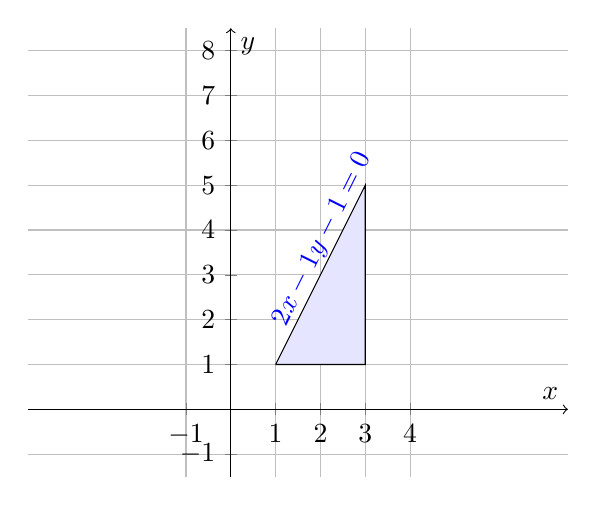
\begin{tikzpicture}
    \begin{axis}[
        xlabel=$x$,
        ylabel=$y$,
        xmin=-1.5, xmax=4.5,
        ymin=-1.5, ymax=8.5,
        axis lines=middle,
        axis line style={->},
        % ticks=none,
        clip=true,
        xtick={-1,0,1,2,3,4},
        ytick={-1,0,1,2,3,4,5,6,7,8},
        axis equal,
        grid=both,
      ]
      \addplot[fill=blue!10] coordinates {(1,1) (3, 5) (3, 1) (1,1)};
      % \addplot[domain=1:3, blue, dashed] {2*x-1};
      \node[blue, right, rotate=63.435] at (axis cs: 1, 1.7) {$2x-1y-1=0$};
    \end{axis}
  \end{tikzpicture}
  \caption{Область $D$}
  \label{fig:D}
\end{figure}

%%%%%%%%%%%%%% ЗАДАНИЕ №1 %%%%%%%%%%%%%%
%% Условие задания №1
\begin{problem}
Haйти $p_{\xi, \eta} ( x, y) $, функции и плотности распределения компонент. Построить графики функций распределений $F_\xi(x)$ и $F_\eta(y)$. Будут ли компоненты независимыми?
\end{problem}

\begin{sympycode}
C = symbols("C")
p_xi_eta = Piecewise((C, True), (0, ~D))
int1 = integrate(integrate(p_xi_eta, (y, y_interval_by_x)), (x, x_interval))
C1 = solve(int1 - 1, C)[0]
\end{sympycode}

%% Решение задания №1
\begin{proof}
  Равномерное распределение задаётся следующей плотностью:
  \[
    p_{\xi, \eta} (x, y) = \begin{cases}
      C, & \text{если } (x, y) \in D, \\
      0, & \text{иначе}.
    \end{cases}
  \]
  Найдём константу $C$:
  \[
    \begin{aligned}
      1 & = \iint\limits_{D} p_{\xi, \eta} (x, y) \, dx \, dy
      = \int\limits_{\sympy{x_interval.start}}^{\sympy{x_interval.end}} \, dx \int\limits_{\sympy{y_interval_by_x.start}}^{\sympy{y_interval_by_x.end}} C \, dy
      = \sympy{int1},                                         \\
      C & = \sympy{C1}.
    \end{aligned}
  \]

  Таким образом, плотность распределения равна:

  \[
    \begin{aligned}
      p_{\xi, \eta} (x, y)
       & =
      \begin{cases}
        \sympy{C1}, & \text{если } x \in \sympy{x_interval}, y \in \sympy{y_interval_by_x} \\
        0,          & \text{иначе}.
      \end{cases}
      \\
       & =
      \begin{cases}
        \sympy{C1}, & \text{если } y \in \sympy{y_interval}, x \in \sympy{x_interval_by_y} \\
        0,          & \text{иначе}.
      \end{cases}
    \end{aligned}
  \]
  \begin{sympycode}
p_xi_eta = C1
p_xi = simplify(integrate(p_xi_eta, (y, 1, 2*x-1)))
p_eta = simplify(integrate(p_xi_eta, (x, (1+y)/2, 3)))
\end{sympycode}

  Найдём плотность распределения компонент:

  \[
    \begin{aligned}
      p_{\xi} (x)  &
      = \int\limits_{-\infty}^{+\infty} p_{\xi, \eta} (x, y) \, dy
      = \int\limits_{\sympy{y_interval.start}}^{\sympy{y_interval.end}} \sympy{p_xi_eta} (x, y) \, dy
      = \sympy{p_xi}, \\
      p_{\eta} (y) &
      = \int\limits_{-\infty}^{+\infty} p_{\xi, \eta} (x, y) \, dx
      = \int\limits_{\sympy{x_interval.start}}^{\sympy{x_interval.end}} \sympy{p_xi_eta} (x, y) \, dx
      = \sympy{p_eta}.
    \end{aligned}
  \]

  \begin{sympycode}
F_xi = integrate(p_xi, (x, x_interval.start, x))
F_eta = integrate(p_eta, (y, y_interval.start, y))
\end{sympycode}
  Найдём функции распределения компонент:

  \[
    \begin{aligned}
      F_\xi
      = \int\limits_{-\infty}^{x} p_{\xi} (t) \, dt
       & = \begin{cases}
             0,            & x < \sympy{x_interval.start}, \\
             \sympy{F_xi}, & x \in \sympy{x_interval},     \\
             1,            & x > \sympy{x_interval.end},
           \end{cases}  \\
      F_\eta
      = \int\limits_{-\infty}^{y} p_{\eta} (t) \, dt
       & = \begin{cases}
             0,             & y < \sympy{y_interval.start}, \\
             \sympy{F_eta}, & y \in \sympy{y_interval},     \\
             1,             & y > \sympy{y_interval.end}.
           \end{cases}
    \end{aligned}
  \]
  \begin{figure}[h!]
    \centering
    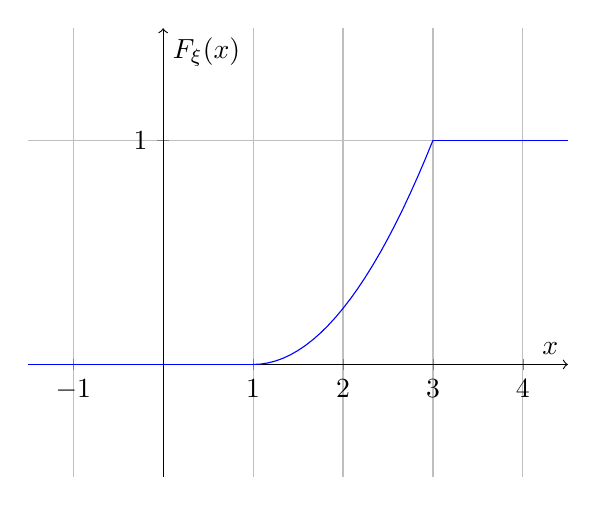
\begin{tikzpicture}
      \begin{axis}[
          xlabel=$x$,
          ylabel=$F_\xi(x)$,
          xmin=-1.5, xmax=4.5,
          ymin=-0.5, ymax=1.5,
          axis lines=middle,
          axis line style={->},
          % ticks=none,
          clip=true,
          xtick={-1,0,1,2,3,4},
          ytick={0,1},
          grid=both,
        ]
        \addplot[domain=-1.5:1, blue, solid] {0};
        \addplot[domain=1:3, blue, solid] {x^2 / 4 - x/2 + 1/4};
        \addplot[domain=3:4.5, blue, solid] {1};
      \end{axis}
    \end{tikzpicture}
    \caption{График функции распределения $F_\xi(x)$}
    \label{fig:F_xi}
  \end{figure}

  \begin{figure}[h!]
    \centering
    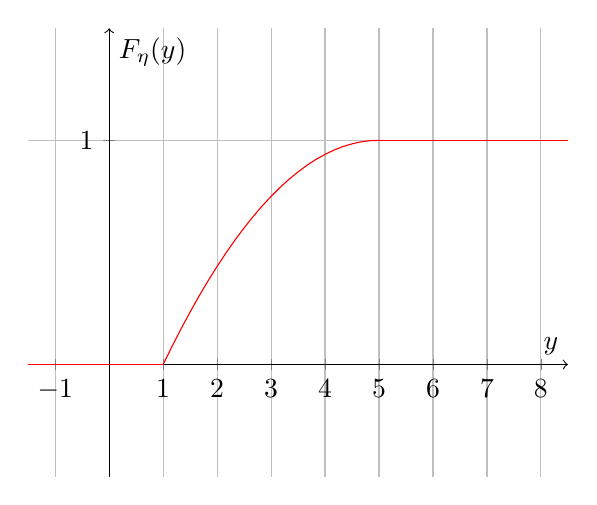
\begin{tikzpicture}
      \begin{axis}[
          xlabel=$y$,
          ylabel=$F_\eta(y)$,
          xmin=-1.5, xmax=8.5,
          ymin=-0.5, ymax=1.5,
          axis lines=middle,
          axis line style={->},
          % ticks=none,
          clip=true,
          xtick={-1,0,1,2,3,4,5,6,7,8},
          ytick={0,1},
          grid=both,
        ]
        \addplot[domain=-1.5:1, red, solid] {0};
        \addplot[domain=1:5, red, solid] {-x ^ 2 / 16 + 5 * x / 8 - 9 / 16};
        \addplot[domain=5:8.5, red, solid] {1};
      \end{axis}
    \end{tikzpicture}
    \caption{График функции распределения $F_\eta(y)$}
    \label{fig:F_eta}
  \end{figure}

  \begin{sympycode}
p_xi_eta_prod = p_xi * p_eta
\end{sympycode}
  Проверка компонент на независимость:

  Для точки $(x, y) \in D$ плотность распределения компонент равна
  \[
    \begin{aligned}
      p_{\xi, \eta} (x, y) & = \sympy{p_xi_eta},                                                                          \\
      p_{\xi, \eta} (x, y) & = p_{\xi} (x) \cdot p_{\eta} (y) = \sympy{p_xi_eta_prod} = \sympy{p_xi_eta_prod.simplify()}.
    \end{aligned}
  \]

  Таким образом, компоненты не являются независимыми.

\end{proof}

